%! TEX root = ../main.tex
\documentclass[main]{subfiles}

\begin{document}
\appendix 
\chapter{インタフェース回路}
\label{sec:appendix_figs}

\begin{figure}[h]
  \centering
  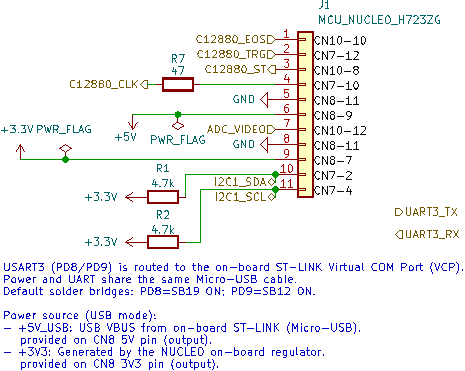
\includegraphics[width=0.8\linewidth]{figures/2/AGV_Multisensor-MCU_NUCLEO_H723ZG.pdf}
  \caption{MCU (NUCLEO-H723ZG) interface circuit}
  \label{fig:mcu_circuit}
\end{figure}

\begin{figure}[h]
  \centering
  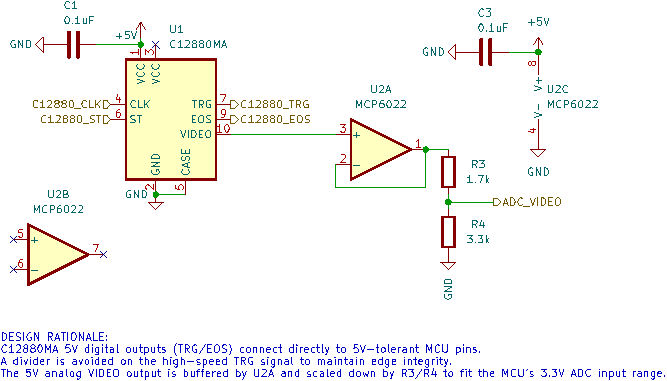
\includegraphics[width=0.8\linewidth]{figures/2/AGV_Multisensor-Spectrometer_C12880MA.pdf}
  \caption{Spectrometer (C12880MA) interface circuit}
  \label{fig:c12880ma_circuit}
\end{figure}

% ===== S300L and BME280 side-by-side =====
\begin{figure}[h]
    \centering
    \begin{subfigure}[b]{0.48\linewidth}
        \centering
        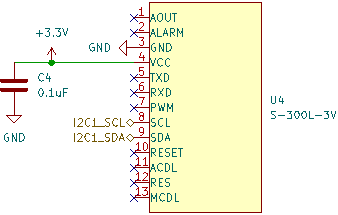
\includegraphics[width=\linewidth]{figures/2/AGV_Multisensor-CO2_S300L.pdf}
        \caption{CO\textsubscript{2} sensor (S300L) interface circuit}
        \label{fig:s300l_circuit}
    \end{subfigure}
    \hfill % Pushes the two figures apart
    \begin{subfigure}[b]{0.48\linewidth}
        \centering
        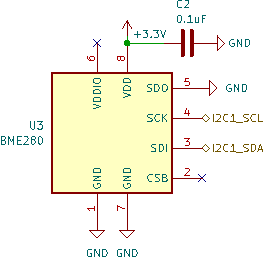
\includegraphics[width=\linewidth]{figures/2/AGV_Multisensor-Env_BME280.pdf}
        \caption{Environmental sensor (BME280) interface circuit}
        \label{fig:bme280_circuit}
    \end{subfigure}
    \caption{Interface circuits for CO\textsubscript{2} and environmental sensors.}
    \label{fig:side_by_side_sensors}
\end{figure}

% \chapter{sensor_unit_code}
%\label{lst:sensor_unit_code}
%\inputminted[linenos,breaklines]{py}{code/a.py}

\end{document}